\section{Beschreibung der aktuellen on-premise BI-Architektur} \label{sec:grundlagen:onpremiseBI}
Die Ausgangslage für die Migration ist ein on-premise betriebenes BI~=System. Dieses ist in der \textit{Hub~=and~=Spoke-Architektur} aufgebaut. Diese gängige Architektur beschreibt die Verwendung eines zentralen Datenspeicherorts (Hub) und darauf aufbauenden, für bestimmte Auswertungen oder Anwendungen optimierte, Datenspeicher (Spokes) \cite{kemper_bi-glossar_2008}. Die Daten aus dem Hub werden also weiterverarbeitet und in den spezialisierten Spokes abgelegt. Abbildung~\ref{fig:aktuelle_onpremise_bi_architektur} zeigt die aktuelle BI~=Architektur, aufgeteilt nach funktionalen Bereichen.
\begin{figure}[htbp]
 \centering
 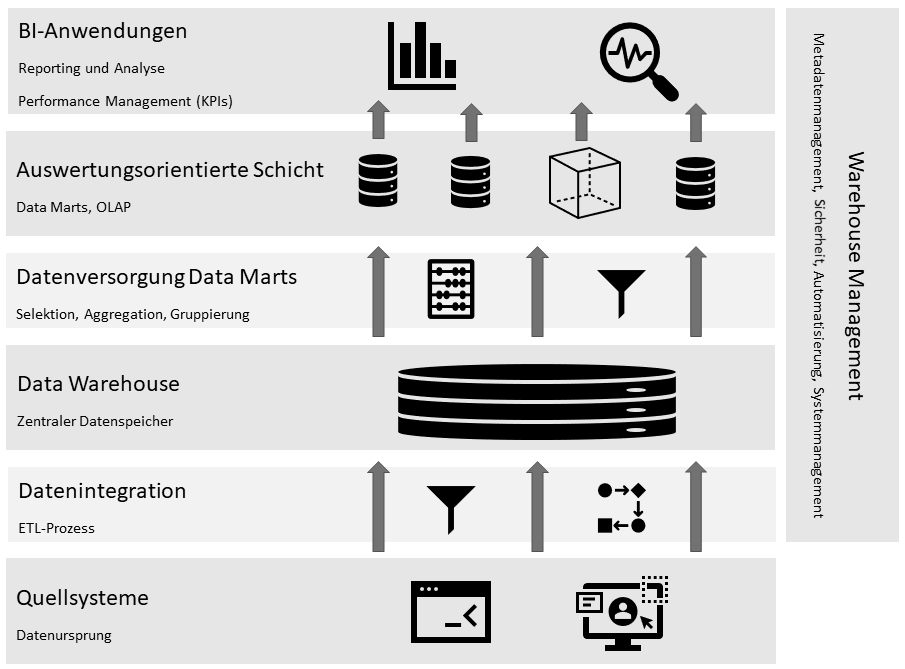
\includegraphics[width=\textwidth]{gfx/aktuelle_onpremise_bi_architektur.png}
 \caption[Aufbau des on-premise BI-Systems]{Aktuelle Architektur des on-premise BI-Systems und Ausgangslage für die Migration in die Cloud \cite{grunwald_business_2009}\cite{humm_architektur_2005}}
\label{fig:aktuelle_onpremise_bi_architektur}
\end{figure}

Die einzelnen Schichten werden im Folgenden erläutert \cite{grunwald_business_2009}\cite{kemper_bi-glossar_2008}\cite{humm_architektur_2005}:
\begin{itemize}
\item \textbf{Quellsysteme} sind der Ursprung aller Daten des BI-Systems. Es kann sich hierbei um interne, sowie externe Quellen handeln. Externe Daten könnten beispielsweise von Marktforschungs- oder Partnerunternehmen stammen. Aktuell sind nur interne Datenquellen angeschlossen. Darunter zum Beispiel die Projektmanagement-Software Jira und das Codeanalyse-Tool SonarQube.
\item Die \textbf{Datenintegration}(auch \ac{etl}) ist die Schnittstelle zwischen dem \ac{dwh} und den Quellsystemen. Der \acs{etl}-Prozess beginnt mit dem Extrahieren von operativen Daten aus einem Quellsystem. Darauf folgt eine Transformation, bei der die Daten an syntaktische Anforderungen angepasst werden und semantische Fehler, wenn möglich, behoben werden. Abschließend werden die Daten in das \ac{dwh} zur Speicherung geladen. Für den \acs{etl}-Prozess werden Funktionen von \textit{Microsofts SQL-Server} und \textit{Powershell-Skripte} genutzt.
\item Das \textbf{Data Warehouse} ist der zentrale Speicherort. Hier werden die Daten strukturiert und langfristig abgelegt. Damit werden sie für weitere Verarbeitungsschritte und Auswertungen zur Verfügung gestellt. In diesem BI-System wird für das Data Warehouse das relationale Datenbankmanagementsystem \textit{Microsoft SQL-Server} verwendet.
\item \textbf{Datenversorgung Data Marts}: Durch den Einsatz von SQL werden in dieser Schicht Bereich Daten selektiert, gruppiert und aggregiert. Das Ziel ist die Aufbereitung der Daten für die Data Marts.
\item \textbf{Auswertungsorientierte Schicht}: Data Marts beinhalten spezialisierte Ausschnitte der Daten aus dem \ac{dwh}, in einer für den Zugriff aus den BI-Anwendungen optimierten Form. Ziel ist es, dass für alle Anwendungsfälle eine effiziente Auswertung ermöglicht wird. Verschiedene Data Marts greifen beispielsweise auf die gleichen Daten mit unterschiedlichem Detailgrad und Selektionskriterien zu. Für komplexere Datenanalysen wird das Konzept des \textit{\ac{olap}} angewendet. Dieses soll es Nutzern ermöglichen, auch ohne technische Kenntnisse, Wissen aus dem \ac{dwh} oder den Data Marts zu extrahieren. Das kann durch die Bereitstellung von Ad-hoc-Reports geschehen, welche eine Benutzeroberfläche besitzen, über die mit einfachen Interaktionen flexible Analysen durchgeführt werden können. Dadurch sind keine Kenntnisse in einer Datenbankabfragesprache, wie SQL, notwendig. Die Grundlage für das \ac{olap} sind die sogenannten \ac{olap} Cubes. Unter diesen wird ein multidimensionaler Datenraum verstanden, bei dem die Dimensionen verschiedenen Kontexte, wie zum Beispiel Produkte, Kunden oder Zeit beschreiben. Sowohl die Data Marts als auch die \ac{olap} Cubes sind entweder als View auf das \ac{dwh} oder als eigenständige Datenbanktabelle realisiert.
\item \textbf{BI-Anwendungen} sind die Benutzerschnittstelle zum BI~=System. Hier erfolgen Auswertung und Präsentation. Im aktuellen BI~=System existieren drei Reporting-Anwendungen, die jeweils eine andere Management~=Ebene als Zielgruppe haben. Von den verschiedenen Arten an BI~=Anwendungen werden die Kategorien \textit{Reporting und Analyse} und \textit{Performance Management} abgedeckt. Bei der ersten Kategorie werden standardisierte Berichte in Form von Listen, Tabellen und Grafiken zur Verfügung gestellt. Beim {Performance Management} wird die Unternehmensleistung anhand von ausgewählten \acp{kpi} dargestellt und mit Zielwerten verglichen. Die vorhandenen BI-Anwendungen wurden mit einem internen Reporting~=Framework entwickelt, das auf dem Web~=Framework AngularJS und einer Java"-script Bibliothek zum Erstellen von Visualisierungen basiert.
\item Das \textbf{Warehouse Management} umfasst Aufgaben bezüglich Aufbaus, Pflege und Betrieb des BI-Systems:
\begin{itemize}
\item \textit{Metadatenmanagement}. Verwaltung von Metadaten und Bereitstellung einer gemeinsamen Metadatenbasis für alle Komponenten im System.
\item \textit{Sicherheit}. Authentifizierung und Autorisierung von Benutzern.
\item \textit{Automatisierung}. Event- oder zeitbasierte Ausführung von Prozessen im \ac{dwh}. Zum Beispiel das Ausführen eines ETL-Prozesses zu einer festen Uhrzeit.
\item \textit{Systemmanagement}. Betrieb des \ac{dwh}s gewährleisten. Dazu gehört zum einen die Überwachung von Performance und Auslastung des Systems und zum anderen die Archivierung und Sicherung von Daten.
\end{itemize}
\end{itemize}